[5~v\textsuperscript{o}] discriminis, ni fallor, quod arcus\protect\index{Sachverzeichnis}{arcus} agit tota vi\protect\index{Sachverzeichnis}{vis} \edtext{determinata eo momento}{\lemma{determinata}\Bfootnote{\textit{(1)}\ statim \textit{(2)}\ eo momento \textit{L}}} quo a projecto deseritur, qui ictus\protect\index{Sachverzeichnis}{ictus} ob moram non increscit. At in Sclopeto\protect\index{Sachverzeichnis}{sclopetum} non primo momento omnis consumitur ictus\protect\index{Sachverzeichnis}{ictus} pulveris, sed absolvitur displosio. Sed nondum ista satisfaciunt. Fiat ergo Experim. 5.
\pend
\count\Bfootins=1200
\pstart
(5) Observetur an oriatur differentia, si pila\protect\index{Sachverzeichnis}{pila} arcu\protect\index{Sachverzeichnis}{arcus} explosa cum chorda adducta fuit, aut si a chorda sub finem restitutionis inventa est. Ego discrimen subesse puto nullum. At in Sclopeto\protect\index{Sachverzeichnis}{sclopetum} alia res, nam si Sclopetum\protect\index{Sachverzeichnis}{sclopetum} breve perinde est, ac \edtext{si}{\lemma{}\Bfootnote{si \textbar\ pila\protect\index{Sachverzeichnis}{pila} aut \textit{gestr.}\ \textbar\ sagitta \textit{L}}} sagitta\protect\index{Sachverzeichnis}{sagitta} avolaret arcu\protect\index{Sachverzeichnis}{arcus} nondum plene restituto. Quare et quae moram conciliant, conducunt ictui. Unde patet cur nimia longitudo inutilis sit imo noceat, ubi scilicet restitutio omnis facta est, tunc enim de reliquo mora pilae\protect\index{Sachverzeichnis}{pila} in Sclopeto\protect\index{Sachverzeichnis}{sclopetum} tantum vim\protect\index{Sachverzeichnis}{vis} ejus attritu\protect\index{Sachverzeichnis}{attritus} diminuit.
\pend
\count\Bfootins=1200
\count\Cfootins=1200
\count\Afootins=1500
\vspace{1.5em}
\pstart
%\begin{wrapfigure}[8]{o}{0.32\textwidth}
\centering  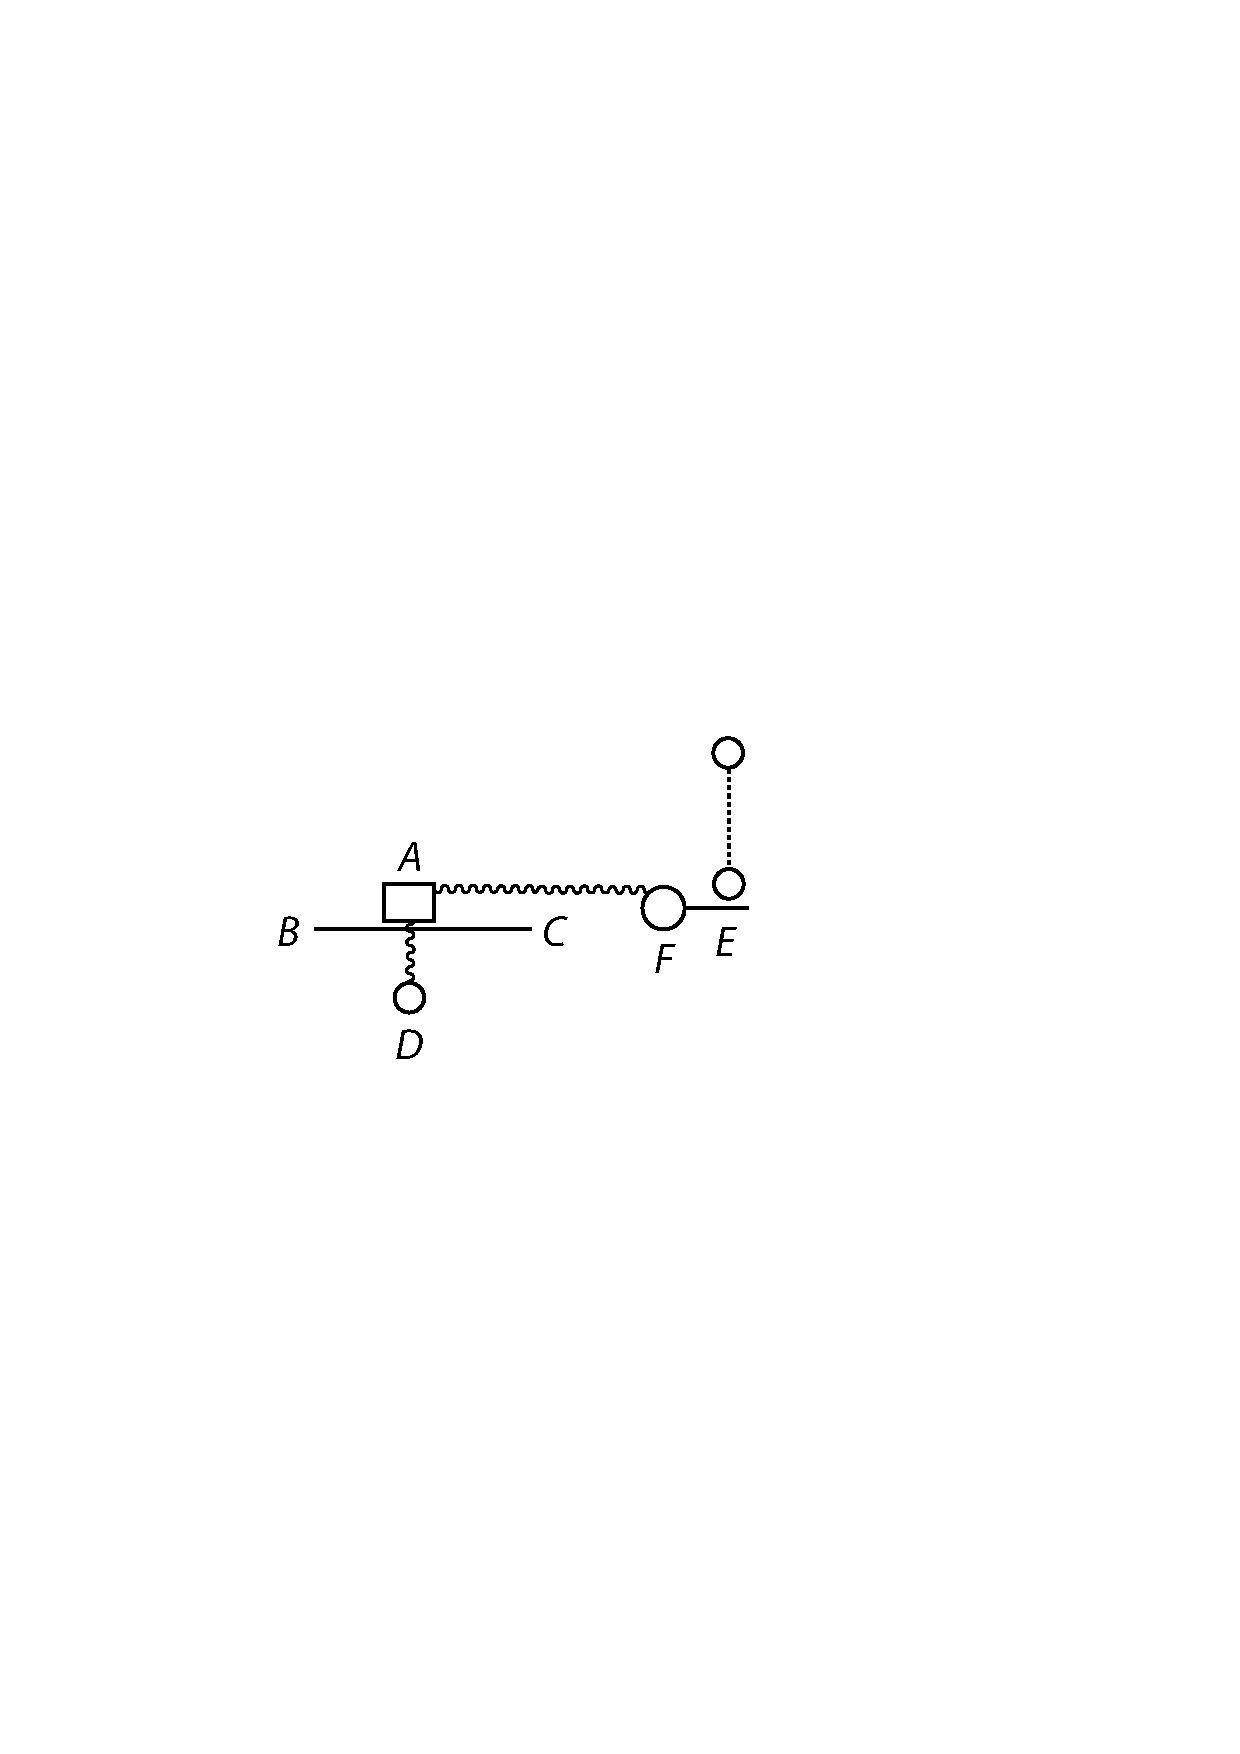
\includegraphics[trim = 0mm 0mm 0mm 0mm, clip, width=0.33\textwidth]{images/lh03705_005v-d1.pdf}\\
    %\caption{Bildbeschreibung}
\noindent \centering [\textit{Fig. 3}] 
    %\end{wrapfigure}
    \pend
    \newpage
\pstart 
  Redeamus ad coepta de\textso{ Detrimento\protect\index{Sachverzeichnis}{detrimentum},} ubi corrigo me, credoque ictum\protect\index{Sachverzeichnis}{ictus} nimis celerem plus etiam difficultatis sentire, in attritu\protect\index{Sachverzeichnis}{attritus} superando. Explicetur \edtext{gluten corporis \textit{A} ad planum \textit{BC}, per}{\lemma{\hspace{-1mm}gluten}\Bfootnote{\hspace{-1mm}\textit{(1)}\ , ope \textit{(2)}\ corporis [...] \textit{BC},  \textit{(a)}\ ope \textit{(b)}\ per \textit{L}\hspace{-3mm}}} pondus quo corpus \textit{A} retinetur in eo loco, quod si jam impellitur quanto celerior est ictus\protect\index{Sachverzeichnis}{ictus} [tanto]\edtext{}{\Bfootnote{\hspace{-2mm}quanto \textit{L \"{a}ndert Hrsg.}\hspace{-3mm}}} celerius ascendet pondus \textit{D}, at [quanto]\edtext{}{\Bfootnote{quan\-do \textit{L \"{a}ndert Hrsg.}\hspace{-3mm}}} pondus 
\textit{D} celerius ascendit tanto resistit magis. At hinc sequitur paradoxum, nimirum majore ictu\protect\index{Sachverzeichnis}{ictus} minus effici. Idque quodammodo verum est, sed recte \edtext{explicandum. Sane}{\lemma{explicandum.}\Bfootnote{\textit{(1)}\ Ajo ergo: Si vis
 impressa\protect\index{Sachverzeichnis}{vis impressa}, id es \textit{(2)}\ Id est \textit{(3)}\ Sane \textit{L}}} etsi ictus\protect\index{Sachverzeichnis}{ictus} infinitus sit si ponderi comparetur, tamen et resistentia\protect\index{Sachverzeichnis}{resistentia} ponderis tunc fit infinita. 
 Ponamus aliud pondus lapsu suo in \textit{E} circumagere trochleam\protect\index{Sachverzeichnis}{trochlea} \textit{F}, et attrahere corpus \textit{A}, atque allevare pondus \textit{D}. Sane primo impactus momento haud dubie attollet \textit{D}, sed ob \edtext{celeritatem\protect\index{Sachverzeichnis}{celeritas} elevationis, id fortissime}{\lemma{celeritatem}\Bfootnote{\textit{(1)}\ id etiam fo \textit{(2)}\ elevationis, id fortissime \textit{L}}} resistet, citoque omnia in verum redibunt modum depereunte paulatim accessione accelerationis\protect\index{Sachverzeichnis}{acceleratio}. Ponamus jam simpliciter incumbere, quanto Trochlea\protect\index{Sachverzeichnis}{trochlea} \textit{F} major est, tanto \textit{D} difficilius \edtext{elevabitur. Certum est}{\lemma{elevabitur.}\Bfootnote{\textit{(1)}\ Sed r \textit{(2)}\ Certum est \textit{L}}} ergo, quid celeriter impingat in \textit{A}, duo consideranda, \edtext{quantitatem}{\lemma{}\Bfootnote{quantitatem  \textbar\ virtutis \textit{ gestr.}\ \textbar\ agentis, \textit{L}}} \edtext{agentis, et celeritatem\protect\index{Sachverzeichnis}{celeritas}. Quantitatem scilicet difformitatis, et vim restitutionis\protect\index{Sachverzeichnis}{vis restitutionis}.}{\lemma{quantitatem [...] celeritatem [...] Quantitatem [...] vim}\Cfootnote{Anstelle der vier Akkusative sollten Nominative stehen.}} \edtext{Si vis}{\lemma{Si}\Bfootnote{\textit{(1)}\ quantitas \textit{(2)}\ vis \textit{L}}} ipsa seu quantitas \edtext{difformitatis minor}{\lemma{difformitatis}\Bfootnote{\textit{(1)}\ major \textit{(2)}\ minor \textit{L}}} sit pondere \edtext{\textit{D}, aucta utcunque celeritate}{\lemma{\textit{D},}\Bfootnote{\textit{(1)}\ ictus\protect\index{Sachverzeichnis}{ictus}  \textit{(a)}\ minor \textit{(b)}\ major \textit{(2)}\ aucta utcunque celeritate \textit{L}}} attolletur pondus fateor, sed ad certam quandam distantiam, quoniam et fortissime resistet. Imo forte ne attolletur quidem ab ictu\protect\index{Sachverzeichnis}{ictus}, utcunque is sit infinite celerior pondere, quia is et infinitam \edtext{resistentiam sentiet, imo non sentiet: ascensus enim}{\lemma{resistentiam sentiet,}\Bfootnote{\textit{(1)}\ ab ascensu infinito, quem \textit{(2)}\ imo [...] enim \textit{L}}} tantus \edtext{est quanta}{\lemma{est}\Bfootnote{\textit{(1)}\ quantus \textit{(2)}\ quanta \textit{L}}} \edtext{celeritas\protect\index{Sachverzeichnis}{celeritas} impingentis}{\lemma{celeritas}\Bfootnote{\textit{(1)}\ cadentis \textit{(2)}\ impingentis \textit{L}}} in quolibet momento. Imo sentiet. Nam haec celeritas\protect\index{Sachverzeichnis}{celeritas} est infinita ratione primae celeritatis\protect\index{Sachverzeichnis}{celeritas}, qua motus coeptus erat. Ergo concludere mihi posse videor non attolli pondus ob majorem ictus\protect\index{Sachverzeichnis}{ictus} celeritatem\protect\index{Sachverzeichnis}{celeritas}, nisi et vis\protect\index{Sachverzeichnis}{vis} sit major. Distinguenda vis\protect\index{Sachverzeichnis}{vis} a nisu, ut pondus a \edtext{ponderatione. Haec tamen}{\lemma{ponderatione.}\Bfootnote{\textit{(1)}\ Caeterum ex his colligo \textit{(2)}\ Haec tamen \textit{L}}} accuratius excutienda, et ut experimentis stabiliantur:
\edtext{(6)}{\lemma{(6)}\Bfootnote{\textit{erg. L}}}%
\textso{ experiamur }primum, an fortius agat arcus\protect\index{Sachverzeichnis}{arcus} si restitutio integra ei permittatur, quam dimidia, ac de eo primum non \edtext{dubito. Nam ad}{\lemma{dubito.}\Bfootnote{%
\textbar\ Imo dubium subest. \textit{gestr.} \textbar\ Nam %
\textit{(1)}\ corpora \textit{(2)}\ sagittam jam \textit{(3)}\ ad \textit{L}}} se restituendum quolibet momento nova vi\protect\index{Sachverzeichnis}{vis} naturae agitur, etsi ea vis\protect\index{Sachverzeichnis}{vis} sit decrescens. Hoc stabilito, \edtext{(7)}{\lemma{(7)}\Bfootnote{\textit{erg. L}}} emittatur globus ex arcu\protect\index{Sachverzeichnis}{arcus}, ac primum ex arcu\protect\index{Sachverzeichnis}{arcus} parum, deinde ex arcu\protect\index{Sachverzeichnis}{arcus} integre restituto, ita ut ictus dirigatur in \edtext{corpus, ponderis ita temperati}{\lemma{corpus,}\Bfootnote{\textit{(1)}\ quod \textit{(2)}\ tanti \textit{(3)}\ ponderis ita temperati \textit{L}}}, ut paulo minor sit vis\protect\index{Sachverzeichnis}{vis} ejus vi\protect\index{Sachverzeichnis}{vis} arcus\protect\index{Sachverzeichnis}{arcus} integre tensi, \edtext{vel restituti}{\lemma{}\Bfootnote{vel restituti \textit{erg.} \textit{L}}}, paulo major vi\protect\index{Sachverzeichnis}{vis} arcus\protect\index{Sachverzeichnis}{arcus}\textso{ ex parte tensi }vel ex parte restituti, vel brevius chorda arcus\protect\index{Sachverzeichnis}{arcus} in pondus agat. Quod si jam ista Hypothesis vera est, sequitur, chordam non superare pondus, \edtext{nisi vis arcus}{\lemma{nisi}\Bfootnote{\textit{(1)}\ pondus \textit{(2)}\ vis restitutionis\protect\index{Sachverzeichnis}{vis restitutionis} \textit{(3)}\ vis arcus \textit{L}}} eo momento adhuc vi\protect\index{Sachverzeichnis}{vis} ponderis major est; nec considerabitur quod ab acceleratione\protect\index{Sachverzeichnis}{acceleratio} accessit. At si fortior adhuc est, tunc acceleratio\protect\index{Sachverzeichnis}{acceleratio} se faciet sentiri. (Videndum jam an sint obstacula quaedam, quorum resistentia\protect\index{Sachverzeichnis}{resistentia} non augeatur celeritate\protect\index{Sachverzeichnis}{celeritas} impingentis. Et esse arbitror nulla.) \textso{Imo} ex his sequitur absurdum, quod scilicet corpus cadens aliud aequiponderans, aut non multum praeponderans non attolleret[;] quod est contra \edlabel{LH037,05_5v+8r_1}%
experientiam.\protect\index{Sachverzeichnis}{experientia}%
\edtext{}{{\xxref{LH037,05_5v+8r_1}{LH037,05_5v+8r_2}}%
\lemma{experientiam.}\Bfootnote{%
\textit{(1)}\ Credideram olim ictu aliquo corporis quantulicunque corpus quantulumcunque nonnihil moveri,
quam sententiam nunc retracto jamque ad speculationem quandam redeo, olim a me intermissam:
\textit{(2)}\ Credebam [...] invenio. \textit{L}}} [8~r\textsuperscript{o}]
\pend
\count\Bfootins=1500
\count\Cfootins=1500
\pstart
\vspace*{3mm} % PR: proivisorisch